\documentclass[12pt, letterpaper]{article}
\usepackage{graphicx} % Required for inserting images
\usepackage[utf8]{inputenc}
\usepackage{tikz}
\usetikzlibrary{arrows.meta}
\date{June 2025}
\setlength{\parskip}{1em}
\setlength{\parindent}{0em}
\renewcommand{\thesection}{\Roman{section}}
\renewcommand{\thesubsection}{\arabic{subsection}}
\renewcommand{\thesubsubsection}{\alph{subsubsection}}
\newcommand{\tortoise}{\textit{t}}
\newcommand{\hare}{\textit{h}}
\begin{document}
\title{Floyd's Tortoise And Hare}
\author{Huiri Chen}

\maketitle

\section{Introduction}  
In the field of computer science, especially in the study of data structures and algorithms, efficiently detecting cycles in data sequences is a fundamental problem. Floyd's Tortoise and Hare algorithm, also known as the cycle detection algorithm, provides a clever and efficient solution to this problem. Developed by Robert W. Floyd in 1967, the algorithm is both time-efficient and memory-efficient, requiring only constant space and linear time.

The central idea of the algorithm involves using two pointers that traverse a sequence at different speeds — a "tortoise" that moves one step at a time, and a "hare" that moves two steps at a time. If there is a cycle in the sequence, the fast-moving hare will eventually meet the slow-moving tortoise within the cycle. This approach is widely used in detecting cycles in linked lists and in various applications such as functional graph traversal and pseudo-random number generation.

In this document, we will explore the theory behind Floyd's Tortoise and Hare algorithm, walk through an implementation, analyze its performance, and discuss its applications and limitations.

\section{Singly Linked List}
\subsection{Linked List}
As we have known, a singly linked list is a linear collection of data elements whose order is not given by their physical placement in memory. Instead, each element points to the next. Each element is a node, which in its most basic form contains data and a reference to the next node.

Visualization:
\begin{center}
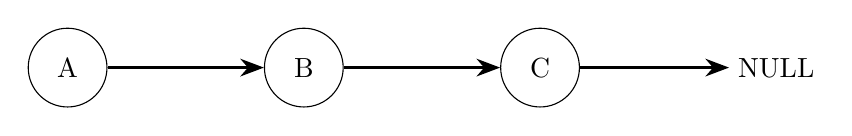
\begin{tikzpicture}[
  node/.style={draw, circle, minimum size=1cm},
  pointer/.style={draw, -{Stealth[length=3mm]}, thick}
]

% Nodes
\node[node] (n1) at (0,0) {A};
\node[node] (n2) at (3,0) {B};
\node[node] (n3) at (6,0) {C};
\node at (9,0) {NULL};

% Arrows
\draw[pointer] (n1) -- (n2);
\draw[pointer] (n2) -- (n3);
\draw[pointer] (n3.east) -- (8.4,0);

\end{tikzpicture}
\end{center}
\subsection{FLoyd's Tortoise and Hare}
\subsubsection{Cycle}
First, let us consider this example: Given that we have node A that points to node B, node B points to node C, and node C points back to node A. We can notice that when we traverse any linked list that contains these three nodes , we can never reach the endpoint (nullptr) since we are stuck on path \( A \rightarrow B \rightarrow C \rightarrow A\rightarrow \cdots \) This path is called a cycle.
In general, a cycle is a path that starts at node N and, after traversal, returns back to node N. To be more specific, a path: \( N_1 \rightarrow N_2 \rightarrow \cdots \rightarrow N_n \rightarrow N_1 \) that when we start traversing from any node in it, we will always return back to that node, is called a cycle.

Visualization:
\begin{center}
\begin{tikzpicture}[
  node/.style={draw, circle, minimum size=1cm},
  pointer/.style={draw, -{Stealth[length=3mm]}, thick}
]

% Nodes
\node[node] (n1) at (0,0) {A};
\node[node] (n2) at (3,0) {B};
\node[node] (n3) at (6,0) {C};

% Arrows between nodes
\draw[pointer] (n1.east) -- (n2.west);
\draw[pointer] (n2.east) -- (n3.west);

% Curved arrow from C back to A (up and around)
\draw[pointer] (n3.north) to[out=60, in=120, looseness=1.8] (n1.north);

\end{tikzpicture}
\end{center}
\subsubsection{Algorithm}
We will start with two pointers \(\tortoise\) and \(\hare\) (shorts for tortoise and hare), both begin at the head of the linked list. Then, we let them traverse the linked list, \(\tortoise\) traverses one node in one step whereas \(\hare\) traverses two nodes in one step. There will be two outcomes:
\begin{itemize}
\item \(\hare\) reaches the end of the singly linked list (nullptr). In this case, there exist no cycles, otherwise \(\hare\) would not have been able to reach nullptr.
\item \(\hare\) and \(\tortoise\) "meet" at some node. This means that there exists a cycle in the linked list, otherwise \(\hare\) would not have been able to meet \(\tortoise\). Then we move one pointer back to the head of the linked list, the other remains where they meet. We let both of them traverse with the speed of one node per step. The node where they meet is the beginning of the cycle.
\end{itemize}
\subsection{Theoretical Background}
FTH works because \(\hare\) traverses the linked list faster than \(\tortoise\), so if there is no cycle and the linked list is a straight path, they will never meet and \(\hare\) will be able to reach the end (nullptr). Only with the help of a cycle can \(\tortoise\) catch up to and meet \(\hare\). Now, i will explain the method we use to detect the beginning of the cycle.

Here is an example linked list for visualization:
Let the number of nodes that are not in the cycle be \(a\) and the number of nodes that are in the cycle be \(b\). 

The number of steps \( \tortoise \) needs to take to enter the cycle is \( a \) steps for the \( a \) nodes it needs to traverse. During that time, \( \hare \) has traversed \( 2 \cdot a \) nodes and has already entered the cycle. We mark the beginning of the cycle with index 0, the nodes after it with \( 1, 2, \cdots, b - 1 \). \( \hare \) is currently at node \( (2 \cdot a - a) \bmod b \) or node \( a \bmod b \) in the cycle.


Now we need to find out at which node do these two pointers meet for the first time, we can get the index of that node by solving this modulus equation:

\begin{equation}
n \bmod b = (c + 2 \cdot n) \bmod b
\end{equation}

with \(n\) is the number of steps \(\tortoise\) needs to take to meet \(\hare\). Or: 

\begin{equation}
n \bmod b = -c \bmod b
\end{equation}

We need to find the smallest \(n\) that satisfies the above equation, that will be:

\begin{equation}
n  = b-c
\end{equation}
This mean after \(a\) steps, the pointer that remains in the cycle will reach the start of the cycle, and so does the other node that start again from the head of the linked list.

In conclusion, the node where they meet again is the beginning of the cycle.
\end{document}
